\chapter{Návrh prvního protoypu}
V této kapitole popisuji návrh prvního prototypu. Tento prototyp byl první realizovanou turbínou, a proto na ní lze najít spoustu i zásadních chyb. I přes to byla stavba této turbíny velkou a neocenitelnou zkušeností.

První prototyp byl navržen pomocí zjednodušené teorie. Hlavním zdrojem informací tehdy byly internetové stránky \cite{ve:ve}. 

Jelikož se jednalo o první turbínu, byl záměrně zvolen hodně malý průměr – 1,5~m. Tento průměr se ukázal pro první pokusy jako ideální. Dobře se s touto velikostí pracuje. Při údržbě není s trochou opatrnosti problém manipulovat se složenou turbínou i v interiéru.

\begin{figure}[H]
	\centering
	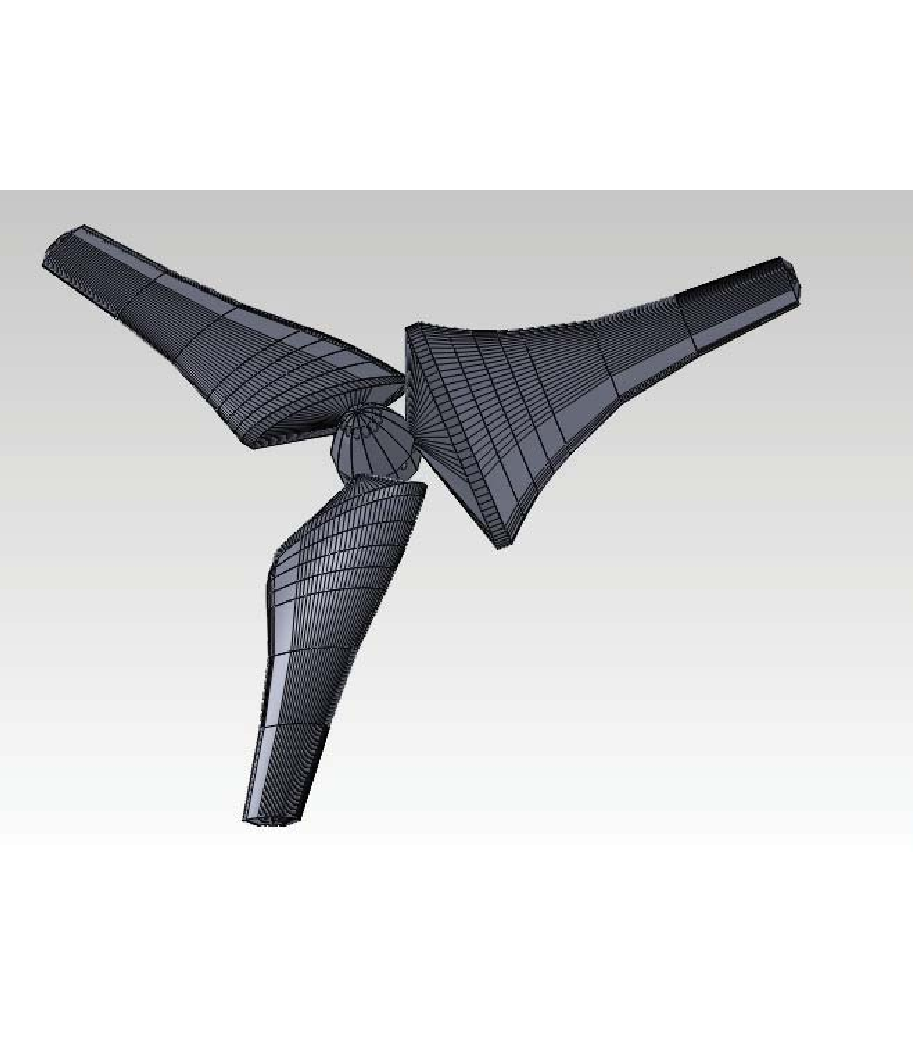
\includegraphics[]{obrazky/prot1p}
	\caption{Pohled na celý CAD model prvního prototypu}
	\label{prot1}
\end{figure}

\begin{figure}[H]
	\centering
	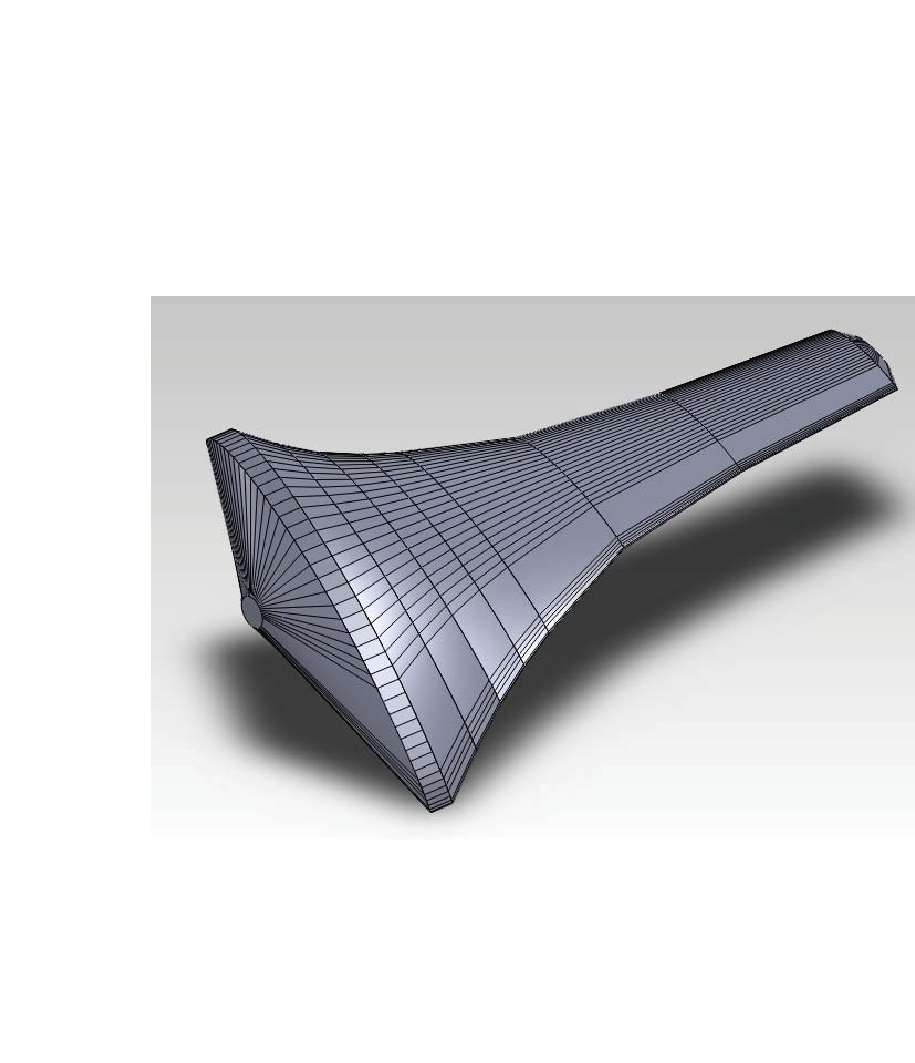
\includegraphics[]{obrazky/prot2p}
	\caption{Pohled na list prvního prototypu}
	\label{prot2}
\end{figure}


Byla také zvolena nízká rychloběžnost turbíny kvůli obavám z hluku. Ty se ukázaly po více než ročním provozu jako neopodstatněné. Nízká rychloběžnost však přinesla jeden neočekávaný negativní efekt. Při nižší rychlosti větru se i turbína otáčí relativně pomalu a vrhá mihotavý stín, který může působit rušivě. Při silnějším větru se však stín přestává mihotat a jeví se jako polostín. Z tohoto důvodu byla při novém návrhu turbíny použita rychloběžnost 5.


Byl použit profil SG6043. Profil byl vybrán hlavně díky jeho vzhledu a jemnosti. Nebyl dále nějak zkoumán. Shodou okolností se později ukázalo, že tento profil je pro použití na větrné turbíně velmi vhodný.

Pro výpočet byl list rozdělen na 7 částí. U osy otáčení byly použity 4 části s tloušťkou 3 cm, jelikož blízko osy otáčení je změna délky tětivy a úhlu náběhu velká. Naopak ke konci listu se tyto změny snižují, a proto byly použity části s~tloušťkou 9, 12 a 15~cm. Pro každou tuto část byl vypočten úhel náběhu a délka tětivy. Následně byly tyto průřezy lineárně spojeny. Na základě těchto dat jsem vytvořil CAD model složený z jednotlivých částí (obrázek \ref{prot1}).

Listy byly zakončeny malým obloukem. Pro navázání na náboj byla přidána jedna část o~tloušťce 1~cm, která má stejnou délku tětivy i úhel náběhu jako předchozí. Na ni navazuje třícentimetrová část, která se sbíhá do kruhu o průměru 2 cm.

Na obrázcích CAD modelu (\ref{prot1} a \ref{prot2}) si lze všimnout největší chyby v návrhu, která v~podstatě znemožnila použití této turbíny pro zisk energie. Je prohozená tlaková a podtlaková strana profilu. Při návrhu jsem se příliš inspiroval klasickými leteckými vrtulemi, které fungují přesně naopak – proud vzduchu urychlují, nikoliv jej zpomalují.

Tato chyba výrazně snižuje podávaný výkon a účinnost této turbíny. Avšak díky použitému profilu neznemožnila zcela funkci turbíny. Při pohledu na graf průběhu součinitele vztlaku v~závislosti na úhlu náběhu (graf \ref{graf:zavislost1}) lze zjistit, že při neoptimálním úhlu náběhu $-5\,^{\circ}$ profil SG6043 stále dosahuje kladné hodnoty součinitele vztlaku. Konkrétně hodnoty 0,36. Součinitel odporu při tomto úhlu náběhu nepatrně vzrostl. Hodnota součinitele vztlaku je $3,5\times$ nižší. Díky tomu turbína dosahuje minimálního výkonu. 






\chapter{Výroba prvního prototypu}
\section{Výroba listů}
V této kapitole popisuji postup a technologii výroby, kterou byly vytvořeny listy prvního prototypu. Dále shrnuji výhody a nevýhody použitého postupu.

Pro výrobu listu bylo nutné zvážit několik požadavků. Prvně je nutné nějakým způsobem dodržet správný tvar. List by měl být vyroben z materiálu, který se dá snadno opracovat a měl by být zvolen postup, kterým jdou vyrobit 3 listy s co nejmenšími odchylkami v jejich tvaru. Dále by měl být použitý materiál co nejlehčí, aby nebyl náboj příliš zatěžován odstředivou silou. List však musí vydržet odpor větru.

Listy jsou vyrobeny ze zbytků zateplovacího polystyrenu. Uvnitř nich je nosná konstrukce složená z ocelové tyče o průměru 10 mm a délce 240 mm (z toho 160 se nachází uvnitř listu). Na tuto kulatinu byla připájena tenčí, pětimilimetrová, kulatina o délce 360 mm, která tvoří výztuhu u konce listu, kde je profil tak tenký, že se zde desetimilimetrová kulatina nevleze. Povrch listů je potažen dvěma vrstvami netkané textilie prosycené lepidlem.

Jednotlivé části listu byly vyříznuty nažhavený drátem (odporový drát připojený na zdroj stejnosměrného proudu) podle připravených šablon z hliníkového plechu. Tyto šablony byly vytvořeny z výše uvedeného CAD modelu. Jejich tvar byl vytištěn na laserové tiskárně a následně přežehlen na hliníkový plech. Tyto šablony pak byly vyříznuty a dobroušeny na požadovaný tvar.

Výroba každé části listu probíhala následovně. Prvně jsem uřízl nažhaveným drátem desku polystyrenu požadované tloušťky. Do ní jsem následně vyvrtal trubkovým vrtákem díru pro nosník. Do díry jsem nasadil pomocný kolík a pomocí něj přilepil oboustrannou lepicí páskou jednu šablonu. Na druhou stranu byla přilepena adekvátní šablona. Jejich vzájemnou pozici určoval kolík v díře pro nosník a pak dále značky vytvořené v CAD modelu. Tyto značky musí s kolíkem ležet v jedné rovině. Tím bylo zajištěno správné zkroucení dané části.

Samotné vyříznutí podle šablon vyžadovalo trochu nácviku a zkoušení. Prvně bylo nutné najít správný proud, který musí drátem téci, aby polystyren řezal, ale nepálil. Dále bylo nutné se naučit, jak drátem táhnout. Problém zde byl v tom, že šablony mají různou velikost a rozdílný obvod. Na jedné straně je tedy nutné drátem táhnout rychleji. To se mi po určitém nácviku nakonec povedlo a~byl jsem schopen řezat bezchybné tvary. Na závěr byly šablony odlepeny pomocí několika kapek technického benzínu, který rozpustil lepidlo lepicí pásky.

Jednotlivé části potom byly slepeny pomocí lepidla UHU por. Části se k sobě lepily nasazené na nosníku, čímž byla zajištěna jejich správná pozice. List byl po slepení přilepen k nosníku. Prvně pomocí lepidla UHU por, to se však ukázalo jako nespolehlivé pro spojení polystyrenu a~kovu. Po několika dnech provozu turbíny jeden z listů vlivem odstředivé síly upadl. Na nosníky proto byla vybroušena plytká drážka ve tvaru spirály a listy byly přilepeny lepidlem Purex. Toto lepidlo při tvrdnutí pění a vyplňuje velký prostor. Proto zateče mezi jednotlivé kuličky polystyrenu a zároveň do drážky na nosníku. Tento spoj se ukázal jako spolehlivý – již přes rok pevně drží.

List byl postupně potažen dvěma vrstvami netkané textilie prosycené lepidlem Herkules. Tato povrchová skořepina dodala listu pevnost a odolnost vůči povětrnostním podmínkám. Původně měl být list ještě natřen epoxidovým lakem pro zvýšení odolnosti. Avšak ani 2 vrstvy netkané textile nejsou dokonale nepropustné a lak se na pokusném listu prosákl dovnitř a rozpustil polystyren. Jak ukázal čas, listy jsou i bez tohoto nátěru dostatečně odolné. List byl na závěr natřen třemi vrstvami bílého latexového nátěru.

Pro statické vyvážení celého rotoru bylo nutné dva listy dovážit olověnými závažíčky o hmotnosti 2 a 1 gram. Tato závažíčka byla přilepena vteřinovým lepidlem. K mému překvapení i po roce provozu stále drží přilepená.

\section{Umístění - gondola, stožár}
Jelikož jediné možné umístění turbíny je na zahrádce, vznikl požadavek na stožár – nesmí mít kotvící lana. Na stožár byl použit 3,5 m dlouhý starý anténní stožár. Pro případnou demontáž není přímo ukotven v zemi.

Do hloubky 1 m byla zabetonována 2 m dlouhá trubka, která slouží jako lože pro stožár. V~případě potřeby je možné tedy stožár z této ukotvené trubky vysunout a schovat. Stožár je v~této trubce jištěn 6 šrouby zašroubovanými do navařených matek. Celé toto kotvení se v~průběhu času ukázalo jako spolehlivé – i při nejvyšší vichřici netrpí základy stožáru nějakými vibracemi.

Gondola, na níž je umístěna turbína, vznikla svařením dvou vinklů k sobě pomocí kolmých kousků pásoviny. Na její spodní stranu bylo přivařeno svislé ložisko, okolo kterého se celá gondola otáčí. Jako ložisko pro samotnou turbínu byl použit starý stejnosměrný elektromotor. Ten byl vložen do gondoly a přitažen kovovými stahovacími páskami. Kormidlo, které řídí natáčení celé gondoly, bylo vyříznuto za plastové desky.

Náboj rotoru byl vytočen z kusu hliníku. Do něj byly vyvrtány díry pro nosníky listů. Na nosníky listů byly vyfrézovány plošky, za které je nosník v náboji přitažen.

Na tento samotný náboj jsem vytvořil ještě kryt. Tento kryt není důležitý z aerodynamického hlediska (u takto malé plochy je jeho přínos minimální), ale má hlavně funkci estetickou a chrání náboj před povětrnostními vlivy. Tento náboj byl vytvořen stejnou technologií jako listy. Vytvořil jsem si 2 šablony z hliníkového plechu. Odporovým drátem jsem si nařezal $30^{\circ}$ výseče. Na tuto výseč jsem nalepil šablony a podle šablony jsem vyřízl část náboje. Následně jsem slepil 12 takto vyříznutých výsečí do plného kruhu. Tím vznikl základní tvar náboje, do kterého jsem ještě vyvrtal otvory pro nosníky listů a otvory pro utažení šroubů. Náboj nebyl potažen netkanou textilií – jeho tvar by se špatně potahoval. Byl pouze natřen latexovým nátěrem. Po roce provozu se nátěr začal mírně loupat a na polystyrenu byla patrná deformovaná místa od UV záření.

\chapter{Zkušenosti s provozem}

První prototyp byl vyroben na přelomu září a října 2010. Stožár i s turbínou byl umístěn 29.~října. Od té doby byla turbíny nepřetržitě v provozu.

První problém nastal dva týdny po instalaci – tehdy, jak jsem zmínil výše, upadlo polystyrenové tělo z nosníku. Po změně lepidla se tento problém již znovu neobjevil.

Zhruba po půlroce se ukázalo vertikální ložisko turbíny jako nespolehlivé. Vlivem změny teplot v něm kondenzovala voda a ložisko zarezlo. Po jeho úpravě funguje spolehlivě.

Další problém se netýkal turbíny samotné, ale jejího uložení. Vlivem povětrnostních podmínek se v září 2011 odlepil jeden permanentní magnet uvnitř motoru použitého jako ložisko a začal drhnout o rotor. Motor vydával skřípavý zvuk. Jelikož však motor nelze použít jako generátor (díky nízkým otáčkám turbíny), stačilo uvolněný magnet vytáhnout.

Celá konstrukce turbíny se během roku provozu osvědčila. Původní obavy z hlučnosti se nepotvrdily. Turbína byla i při sebesilnějším větru tichá. Aby byl vůbec slyšet nějaký hluk, musel člověk stát přímo pod stožárem. Ale i tak nebyl hluk větší než např. šumění listí stromů v okolí.

Velký podíl na tomto faktu může mít použití polystyrenu jako hlavního materiálu – listy jsou díky tomu měkké, a tak nepřenáší chvění na celou konstrukci a chvění to nemůže rezonovat. Listy také nejsou křehké a vydržely i krupobití.

Turbína také vyniká svou startovatelností – může za to mohutná oblast listů blízko osy otáčení. Při prvních pokusech jsem zkoušel s turbínou chodit – i takto pomalý proud vzduchu ji zvládl roztočit.

Stožár se také ukázal jako dostatečně pevný. Jelikož je turbína relativně malá, nebyla použita žádná ochrana proti silnému větru. Při silném větru je patrné, jak se stožár na svém vrcholu lehce kýve, ale jinak nic.

Velmi mě překvapila odolnost použité povrchové úpravy. Celý nátěr vydržel bez většího poškození celý rok. V lednu 2012 jsem provedl preventivní údržbu. Turbína byla sundána a~listy byly znovu natřeny. Na původním nátěru byly místy patrné malé praskliny, u konců listů se několik šupinek odlouplo. Avšak vnější skořepina z netkané textilie nejevila žádné známky poškození.

Bohužel turbínu nešlo díky záměně tlakové a podtlakové strany připojit na generátor a získat nějakou elektrickou energii.
Za celou dobu provozu se turbína stala vyhledávanou atrakcí malých dětí. Nebyly na ni žádné negativní ohlasy.

\begin{figure}[H]
	\centering
	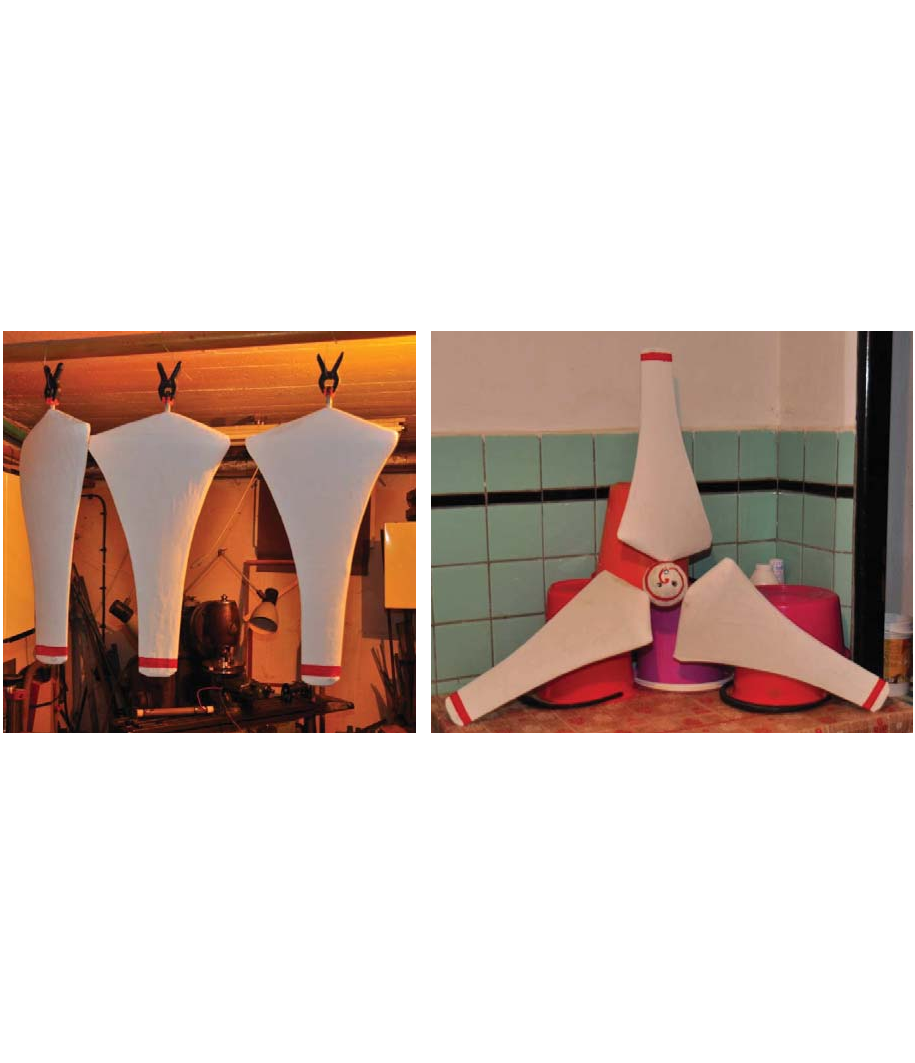
\includegraphics[]{obrazky/foto1}
	\caption{Sušení nově natřených listů při první údržbě v lednu 2012 (vlevo) a pohled na složený rotor (vpravo)}
	\label{foto1}
\end{figure}

\begin{figure}[H]
	\centering
	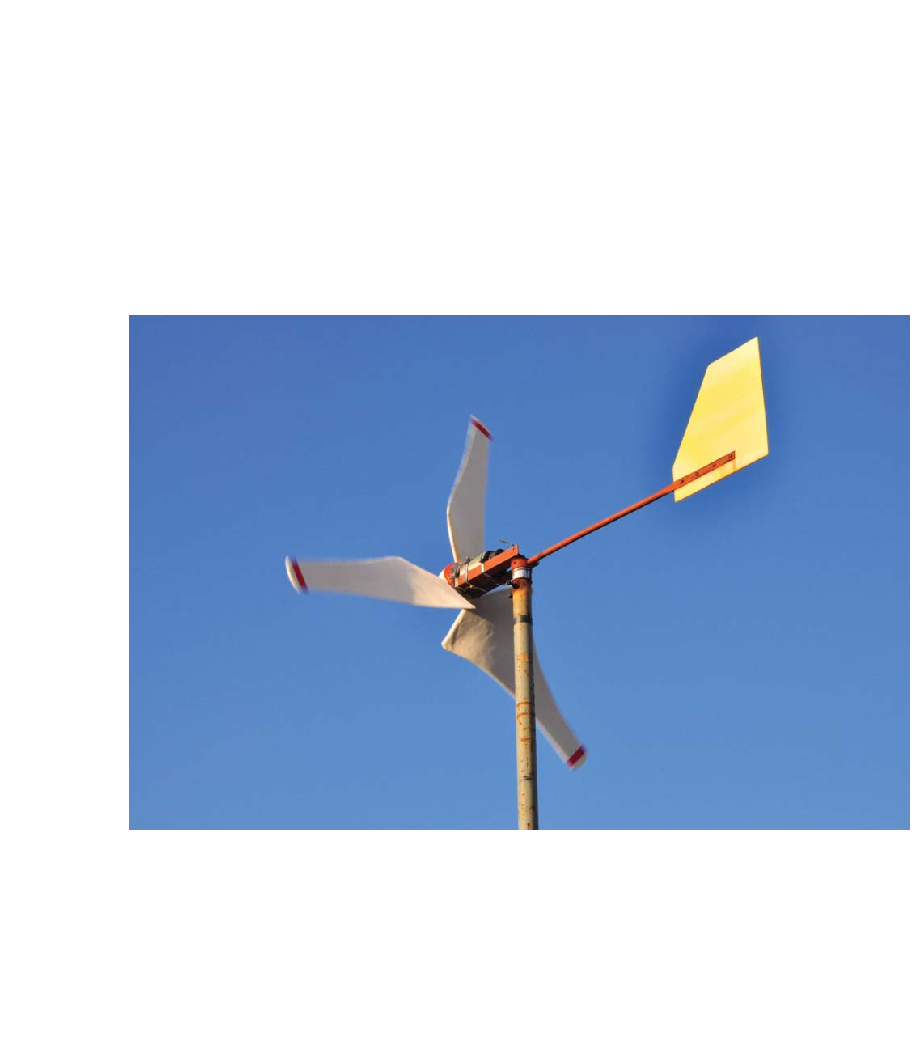
\includegraphics[]{obrazky/foto2}
	\caption{Pohled na celou gondolu}
	\label{foto2}
\end{figure}

\begin{figure}[H]
	\centering
	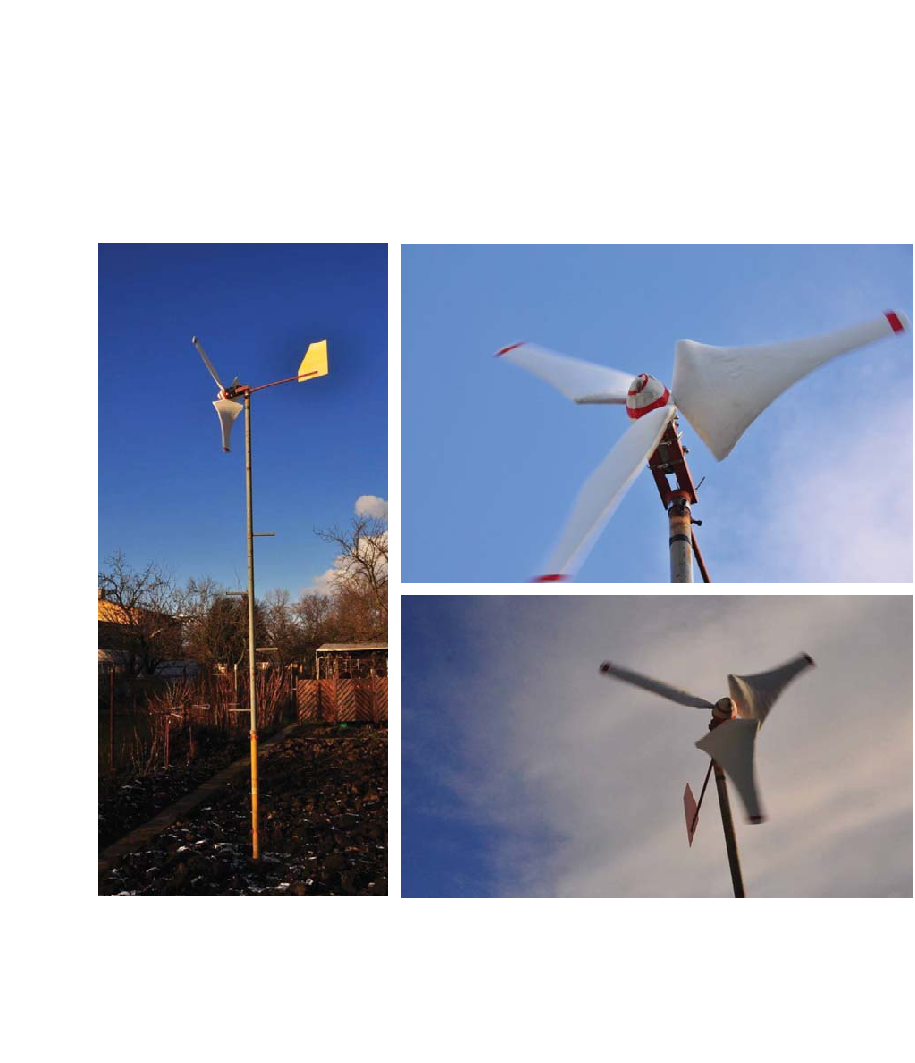
\includegraphics[]{obrazky/foto3}
	\caption{Pohled na stožár (vlevo), pohledy na turbíny při relativně silném větru (vpravo)}
	\label{foto3}
\end{figure}

